% Created 2017-02-24 Fri 17:36
% Intended LaTeX compiler: pdflatex
\documentclass[11pt]{article}
\usepackage[utf8]{inputenc}
\usepackage[T1]{fontenc}
\usepackage{graphicx}
\usepackage{grffile}
\usepackage{longtable}
\usepackage{wrapfig}
\usepackage{rotating}
\usepackage[normalem]{ulem}
\usepackage{amsmath}
\usepackage{textcomp}
\usepackage{amssymb}
\usepackage{capt-of}
\usepackage{hyperref}
\usepackage{indentfirst}
\author{James Nhan, Matt Koenig, Zackery Lovisa, Thien Le, Yue Zhang}
\date{\textit{<2017-02-24 Fri>}}
\title{Augmented Escape}
\hypersetup{
 pdfauthor={James Nhan, Matt Koenig, Zackery Lovisa, Thien Le, Yue Zhang},
 pdftitle={Augmented Escape},
 pdfkeywords={},
 pdfsubject={},
 pdfcreator={Emacs 25.1.1 (Org mode 9.0.2)}, 
 pdflang={English}}
\begin{document}

\maketitle
\begin{align*}
   &\textbf{Target Platform}&&\text{: Microsoft HoloLens} \\
   &\textbf{Target Age}&&\text{: 13+} \\
   &\textbf{Target Rating}&&\text{: T}
\end{align*}

\pagebreak

\tableofcontents

\pagebreak

\section{{\bfseries\sffamily TODO} Story}
\label{sec:org88abcf5}
A mysterious group known only as \emph{The Company} is behind a major conspiracy that will lead to world domination, and you know too much about them. You are being hunted, but death is not your destiny. \emph{The Company} believes anyone can be convinced to join them, and you're no different. They've captured and brough you to a remote location to teach compliance. You will be subjected to various forms of brainwashing and torture techniques. Will you succumb to \emph{The Company}'s will, or will you dash their plans andt take them out from inside?

\section{Characters}
\label{sec:org44a9989}
\subsubsection{{\bfseries\sffamily TODO} Mittens}
\label{sec:org0b4b4f3}
\begin{itemize}
\item Mystical cat.
\item Appears in dire situations to provide help.
\item Requires the player to answer a simple riddle before willing to provide a hint.
\item Has a very playful attitude, making light of the player's current situation
\end{itemize}

\subsubsection{{\bfseries\sffamily TODO} Former Informants}
\label{sec:org2d79e56}
\begin{itemize}
\item Authors of letters that provide backstory for situations.
\item Generic names.
\item Never met by players.
\item Exist solely to introduce scenes.
\end{itemize}

\section{Core Gameplay}
\label{sec:orgf0fd323}
\subsection{{\bfseries\sffamily TODO} Mechanics}
\label{sec:org077fc69}
\begin{itemize}
\item Single player.
\item Puzzle solving.
\item Room is mapped by the HoloLens and augmented to match a scenario.
\item 3-4 puzzles placed around the room randomly.
\item Each puzzle gives a piece of the answer to escaping the current room.
\item Puzzles will be interactable 3D objects in augmented reality.
\item Once all puzzles of a room are solved, their answers can be entered into the door (keys, lock code).
\item Some puzzles and rooms will have random components in order to prevent "trial and error" attempts through the game.
\item Entering a wrong room answer will result in a \textbf{1 minute penalty}.
\item Players will have \textbf{1 hour} to solve all puzzles in all rooms.
\item Scenarios will contain \textbf{3 rooms} each.
\item All rooms must be completed within the time limit to complete the scenario.
\item Upon advancing to a new room in the game, the HoloLens will remap the current room the player is in.
\begin{itemize}
\item The player does not have to change rooms themselves.
\end{itemize}
\item Upon successful completion of the scenario, a story prompt will be shown to the player describing the events that follow the escape.
\item At \textbf{50 minutes} remaining, Mittens will appear to give the players a hint in case they're stuck.
\begin{itemize}
\item If a hint is given, Mittens will disappear and reappear at \textbf{40}, \textbf{30}, \textbf{25}, \textbf{15}, and \textbf{10} minutes remaining.
\item Hints will be consistent for each playthrough of the same scenario.
\end{itemize}
\end{itemize}

\subsection{{\bfseries\sffamily TODO} Goals}
\label{sec:org343f2be}
\begin{itemize}
\item Players win the game if they manage to escape the scenario within an hour.
\item After winning, an expository paragraph will be shown to the player to describe what happens following the escape.
\item Players lose if time expires.
\item After losing, an expository paragraph will be shown to the player to describe what happens to them after their escape fails.
\end{itemize}

\subsection{{\bfseries\sffamily TODO} Hints}
\label{sec:org929091c}
\begin{itemize}
\item Mittens can give the player several types of hints after the player answers a riddle.
\begin{itemize}
\item \textbf{Remove Decoys}: Remove all or some of the decoys in the room.
\item \textbf{Puzzle Explanation}: Explain part of a puzzle to make it easier for the player to solve.
\item \textbf{Answer Location}: Place a glow on an object required for a puzzle.
\end{itemize}
\end{itemize}

\section{Puzzle Types}
\label{sec:org9912620}
\subsection{{\bfseries\sffamily TODO} Acrostic}
\label{sec:org1f9c2c4}
Hint words with numbers under each letter that map to a phrase.

\subsection{{\bfseries\sffamily TODO} Rope Chain}
\label{sec:orgf894ec1}
There will be four \textbf{20 foot} ropes each with four pegs spaced at different distances apart attached along the rope. Only one rope will have the exact peg separation required to insert each peg into four anchored podiums across the room.

\begin{center}
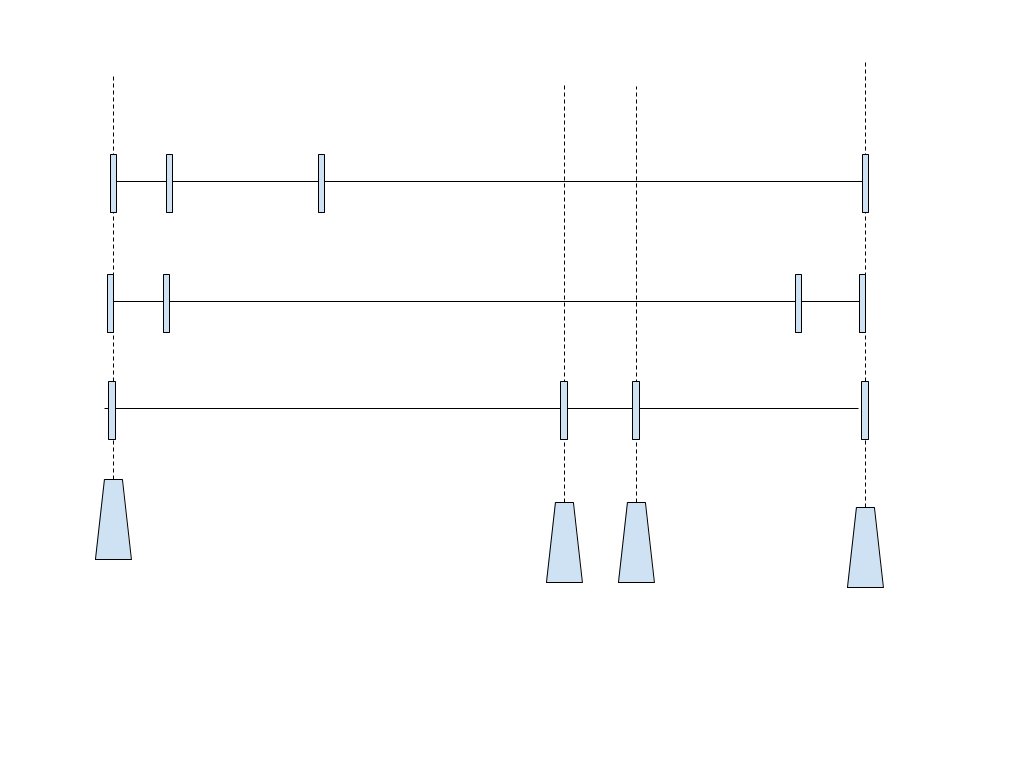
\includegraphics[width=.9\linewidth]{./img/pt-rc-001.png}
\captionof{figure}{\label{fig:org6573fb0}
An example of the ropes, pegs, and podiums.}
\end{center}

\subsection{{\bfseries\sffamily TODO} Block and Key}
\label{sec:org2a1562b}
There will be six \textbf{1 foot} cubes spread across the room. The player will need to place and orient these blocks on a pedestal to create an image by aligning the engravings on each cube. The opposite side of the cube array will then reveal an answer required to escape the room.

\subsection{{\bfseries\sffamily TODO} Cryptogram}
\label{sec:org2f33a5e}
Encrypted messages that need to be put through a cipher in order to be easily read.

\subsection{{\bfseries\sffamily TODO} Connect the Dots}
\label{sec:org61f77b5}
Images drawn may be of other objects in the room. Different shaped dots (e.g. square vs. circle) will connect to make different images. A key will be placed in the room to indicate which dots make the correct image.

\subsection{{\bfseries\sffamily TODO} Statues/Totems}
\label{sec:org64a7339}
\textbf{3-4} statues or obelisks with images need to be positioned in a particular way to unlock an answer. There will be an image depicting how to orient the statues around the room.

\section{References}
\label{sec:org8c8de9f}
\begin{itemize}
\item \href{https://en.wikipedia.org/wiki/Acrostic\_(puzzle)}{Acrostic} - Wikipedia entry.
\item \href{https://en.wikipedia.org/wiki/Cryptogram}{Cryptogram} - Wikipedia entry.
\item \href{http://www.bloodandbones.com/ph12sim/types.htm}{Puzzle Idea List} - A list of puzzle ideas.
\item \href{http://www.accelerated-ideas.com/news/uncharted-4-chapter-1-2-puzzle-solution-rotating-balls.aspx}{Rotating balls and Symbols} - A description of the rotating balls and symbols puzzle from Uncharted 4.
\item \href{http://www.gameshampoo.com/magazine/articles/24/uncharted-3-all-puzzle-solutions.html}{Uncharted 3 All Puzzles} - All of the puzzles in Uncharted 3.
\end{itemize}
\end{document}